\documentclass[UTF8]{beamer}
\usepackage{graphicx, color}
\usepackage{algorithm2e}
\usepackage{zhspacing}
\usepackage{amsmath}
\usepackage{tikz}
\usepackage{url}
\usetikzlibrary{shapes,arrows}

% Define block styles
\tikzstyle{decision} = [diamond, draw, fill=blue!20,
    text width=4.5em, text badly centered, node distance=3cm, inner sep=0pt]
\tikzstyle{block} = [rectangle, draw, fill=blue!20,
    text width=5em, text centered, rounded corners, minimum height=3em]
\tikzstyle{line} = [draw, -latex']
\tikzstyle{cloud} = [draw, ellipse,fill=red!20, node distance=3cm,
    minimum height=2em]

\usepackage{underscore}
\usetheme{JuanLesPins}
\usepackage{fontspec}
\setsansfont{Microsoft YaHei}

\usepackage{enumerate}

\AtBeginSection[]{
  \frame{
    \frametitle{Next}
    \tableofcontents[currentsection, subsectionstyle=show/shaded/hide]
  }
}

\AtBeginSubsection[]{
  \frame{
    \frametitle{Next}
    \tableofcontents[currentsubsection]
  }
}

\title{The World of Programming}

\subtitle{Programming Languages, Methods and Tools}

\author{Gang Chen\\ chengang@genomics.cn}

\logo{
\includegraphics[width=1.3cm]{bgi-logo.png}
\includegraphics[width=2.5cm]{cuhklogo.png}}
\date{\today}




\begin{document}

\begin{frame}
\titlepage
\end{frame}

\begin{frame}[t]\frametitle{Outline}
\tableofcontents[hideallsubsections]
\end{frame}


\section{The World of Programming Languages}

\begin{frame}[t]{The World of Programming Languages}
    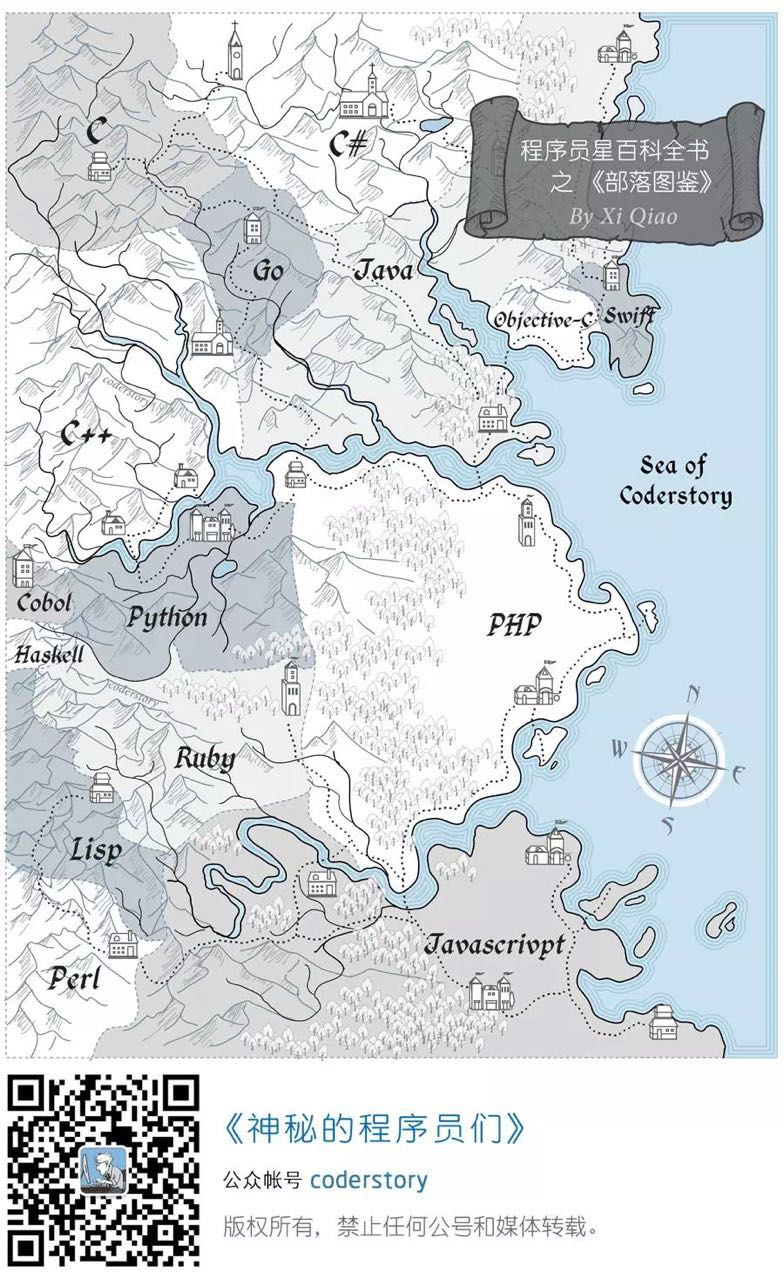
\includegraphics{langworld.jpg}
\end{frame}
%--- Next Frame ---%

\begin{frame}
  \frametitle{Why do we need five programming languages?}
  \begin{block}{Why do we have to learn languages?}
  \begin{itemize}
    \item 廣東話
    \item 普通话
    \item 客家话
    \item 上海话
    \item English
    \begin{itemize}
      \item England, Scotland, Wales, North Ireland
      \item United States
      \item Hong Kong
    \end{itemize}
    \item Hinglish
    \item \ldots
  \end{itemize}
\end{block}
\end{frame}

\begin{frame}
  \frametitle{Programming Languages}
  \tiny
  \begin{itemize}
    \item C: Embedded device, high performance system software
    \item C++: Embedded device, large-scale software, GUI applications
    \item Java: Large-scale system, Enterprise systems, cross-platform applications
    \item Perl: Text processing, biological sequence processing, CGI-programming
    \item Python: System administration, desktop applicatons, web development
    \item R: Data analysis and visualization
    \item Objective-C: applications on iOS and Mac OS
    \item Swift: a future programming languages for Apple products
    \item Go: Google's system programming language
    \item Haskell: Functional Programming language
    \item Ruby, Scala, Julia, JavaScript, LaTeX \ldots
  \end{itemize}
\end{frame}

\begin{frame}
  \centerline{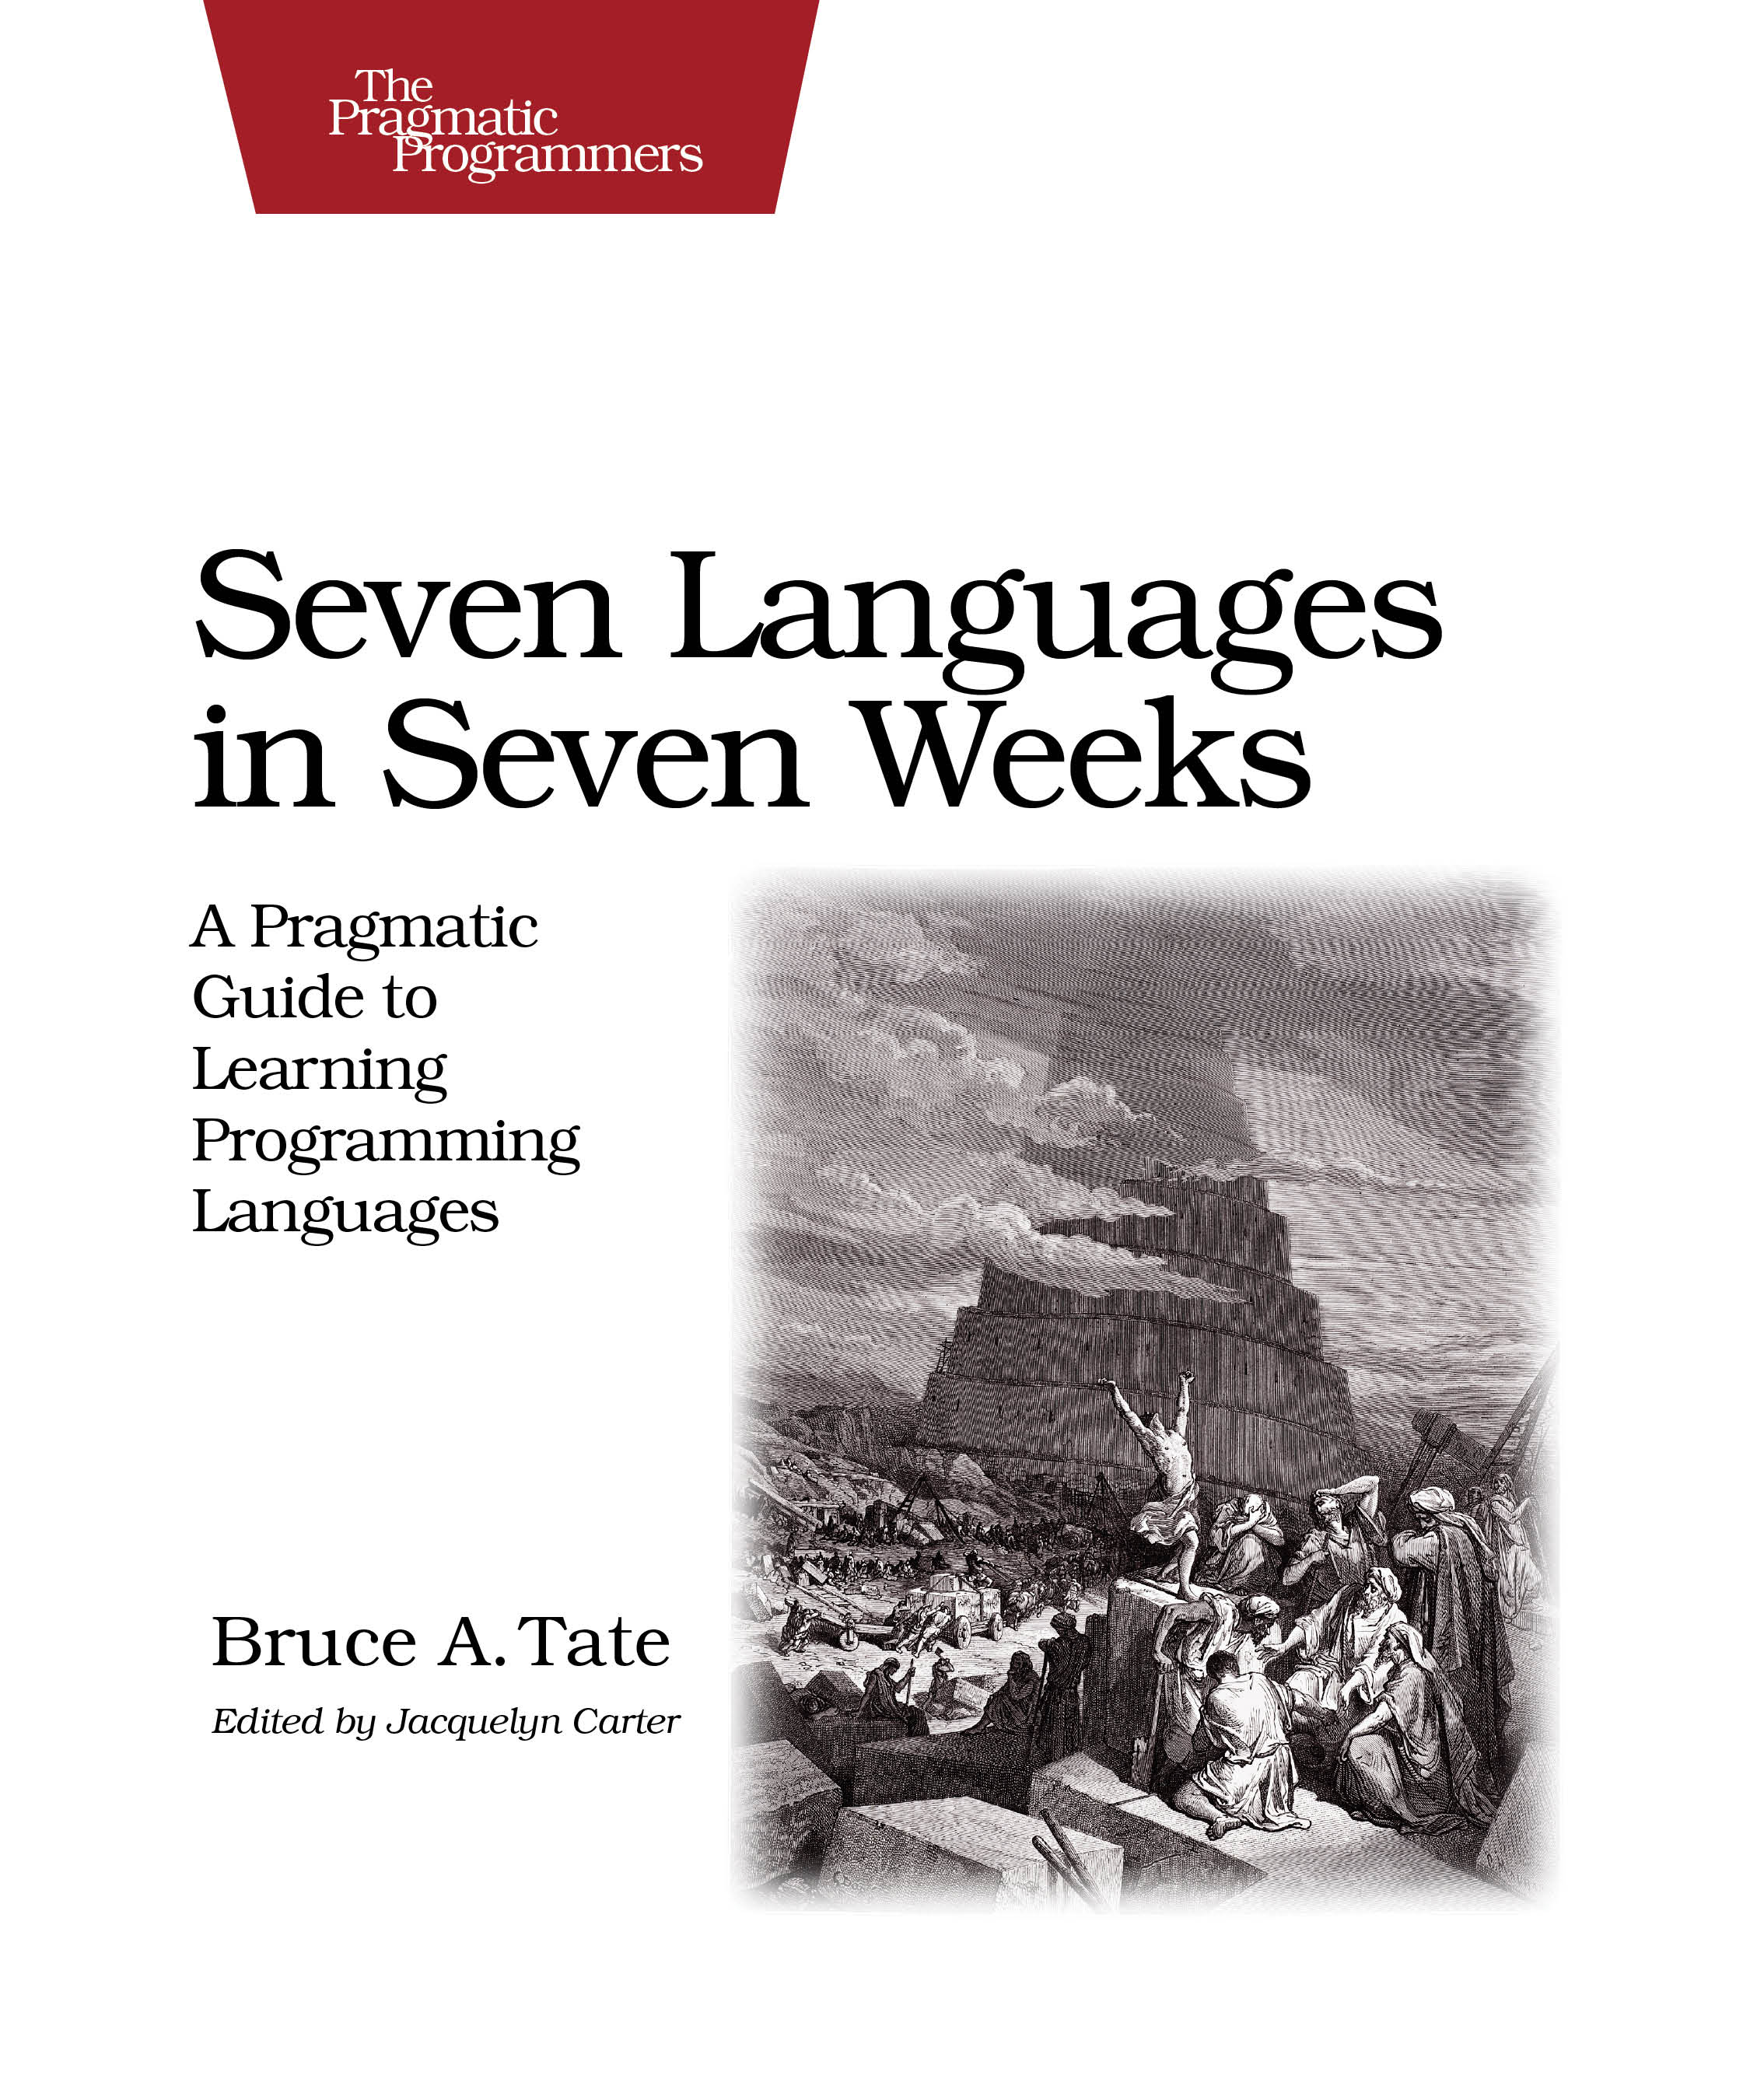
\includegraphics[height=\textheight]{slsw.jpg}}
\end{frame}

\begin{frame}
  \centerline{
\includegraphics[height=\textheight]{smlsw.jpg}}
\end{frame}

\begin{frame}
  \centerline{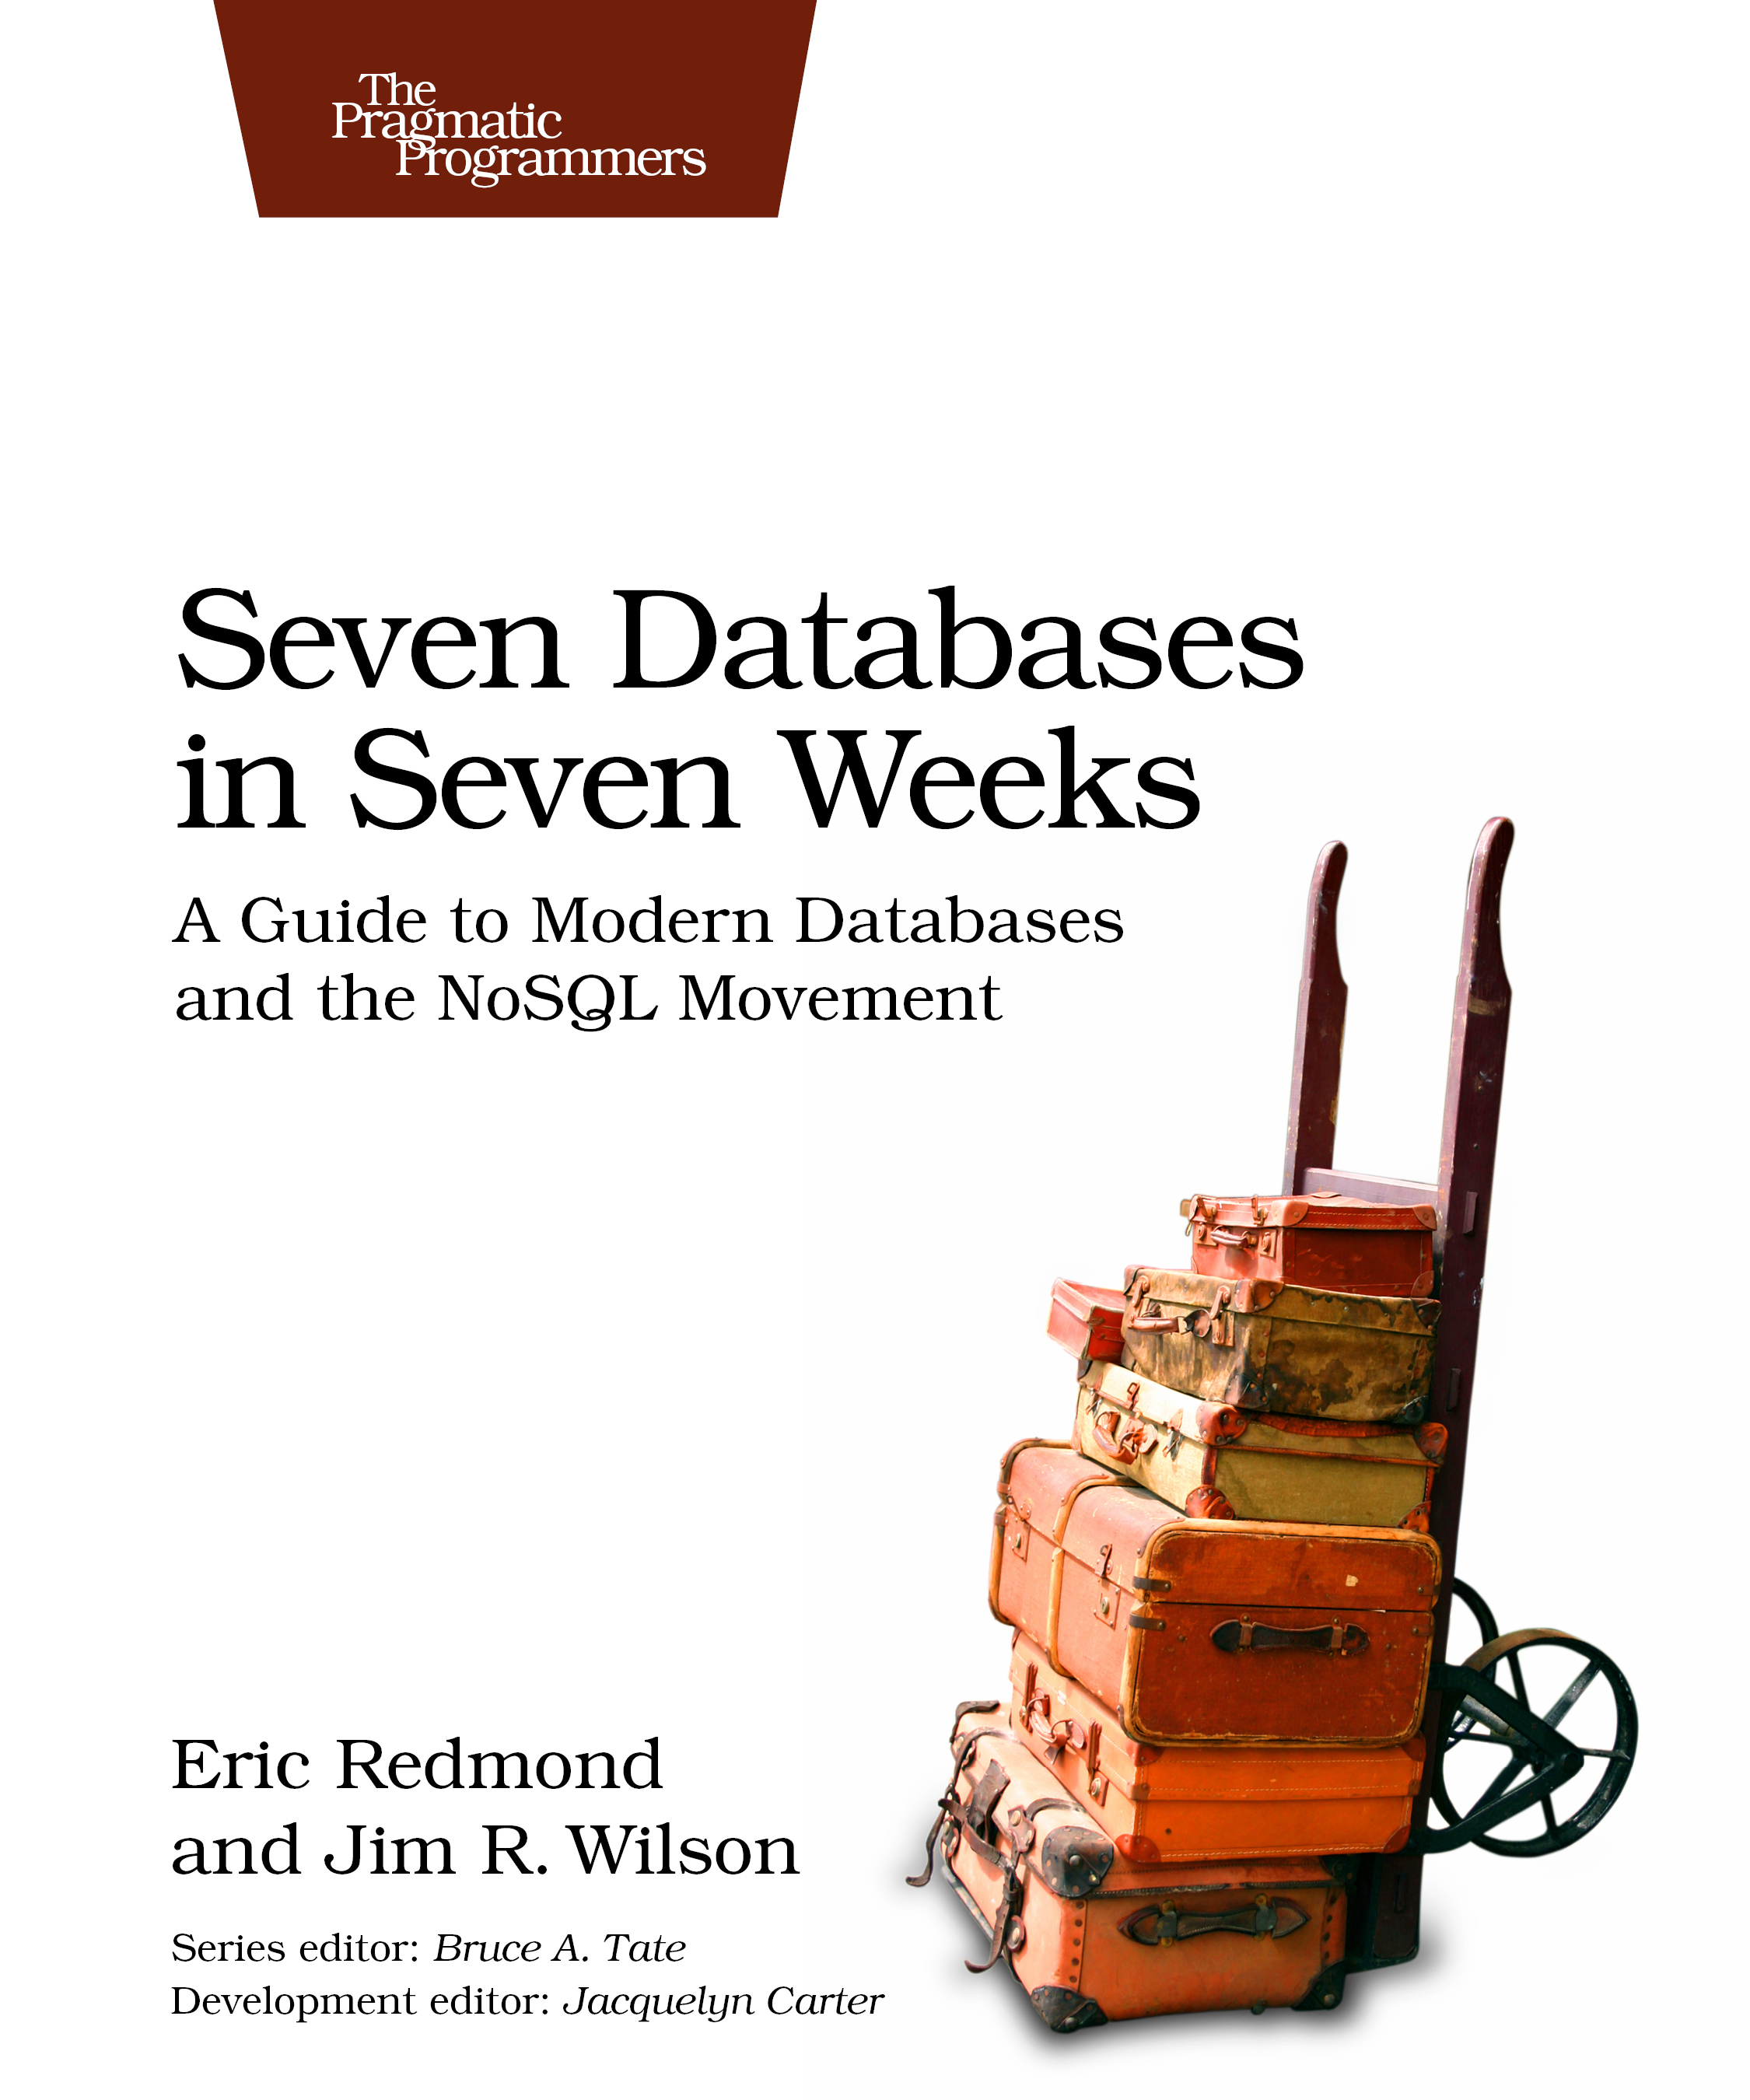
\includegraphics[width=.33\textwidth]{sdsw.jpg}
  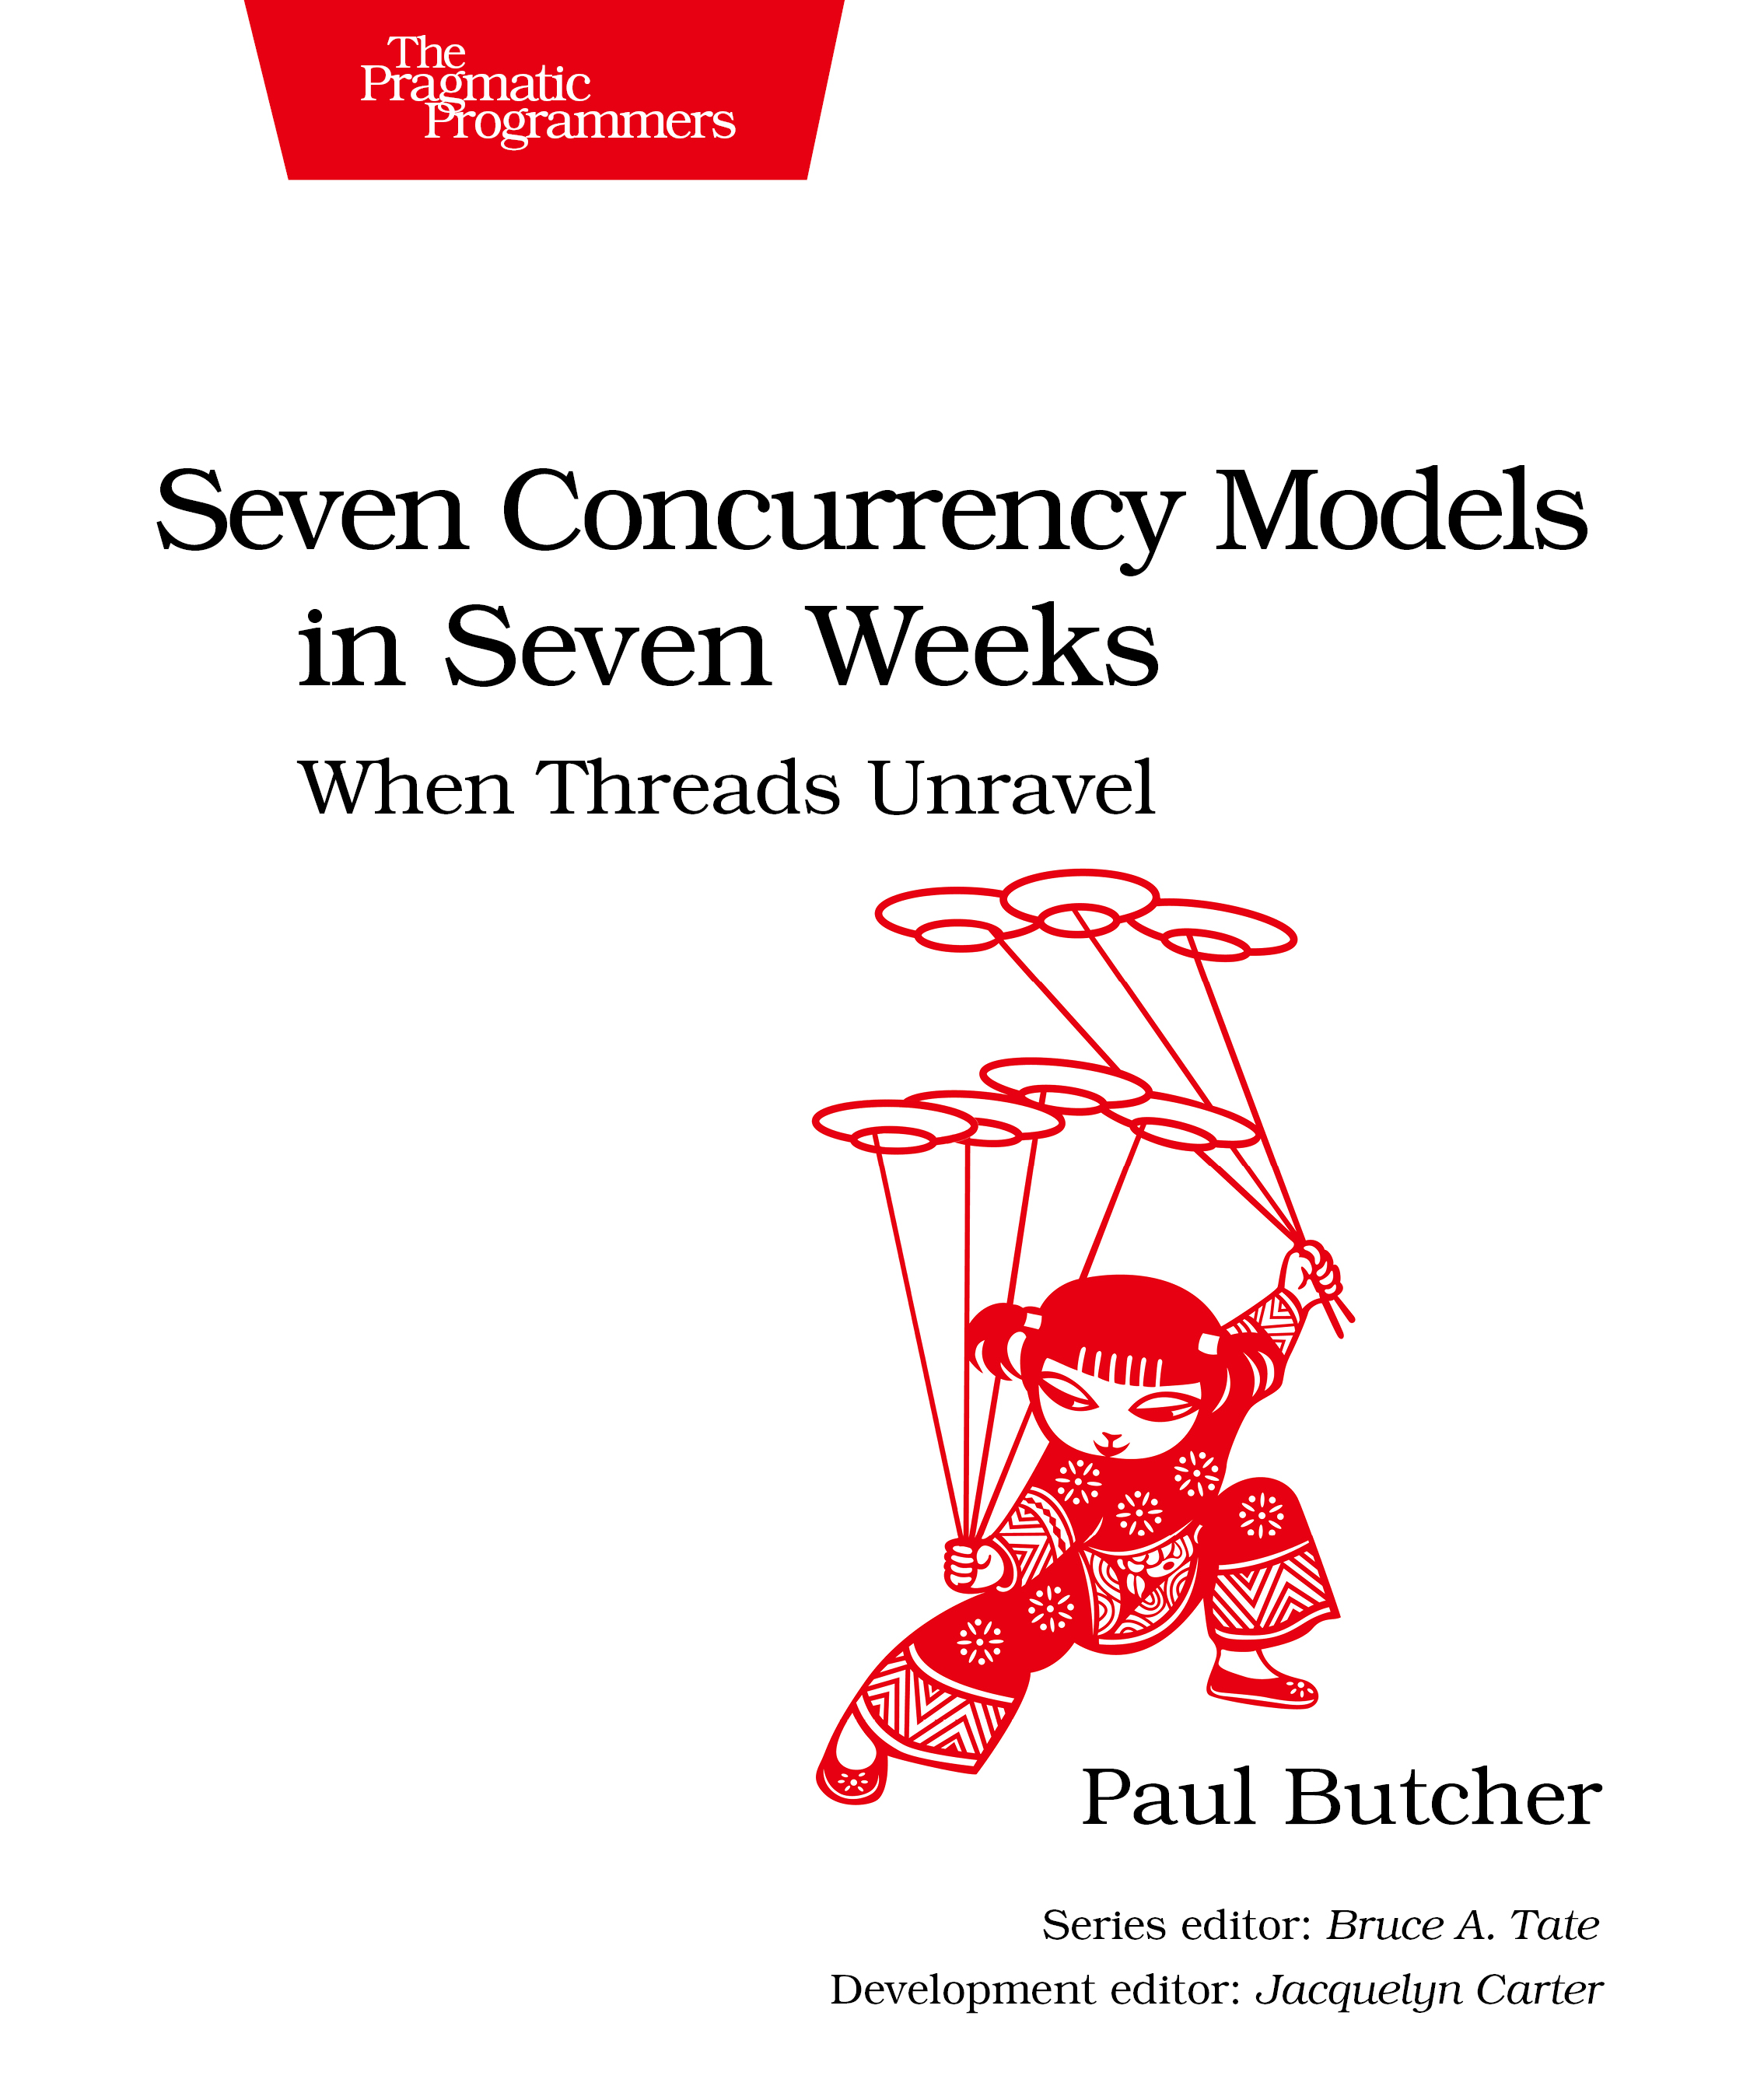
\includegraphics[width=.33\textwidth]{scmsw.jpg}
  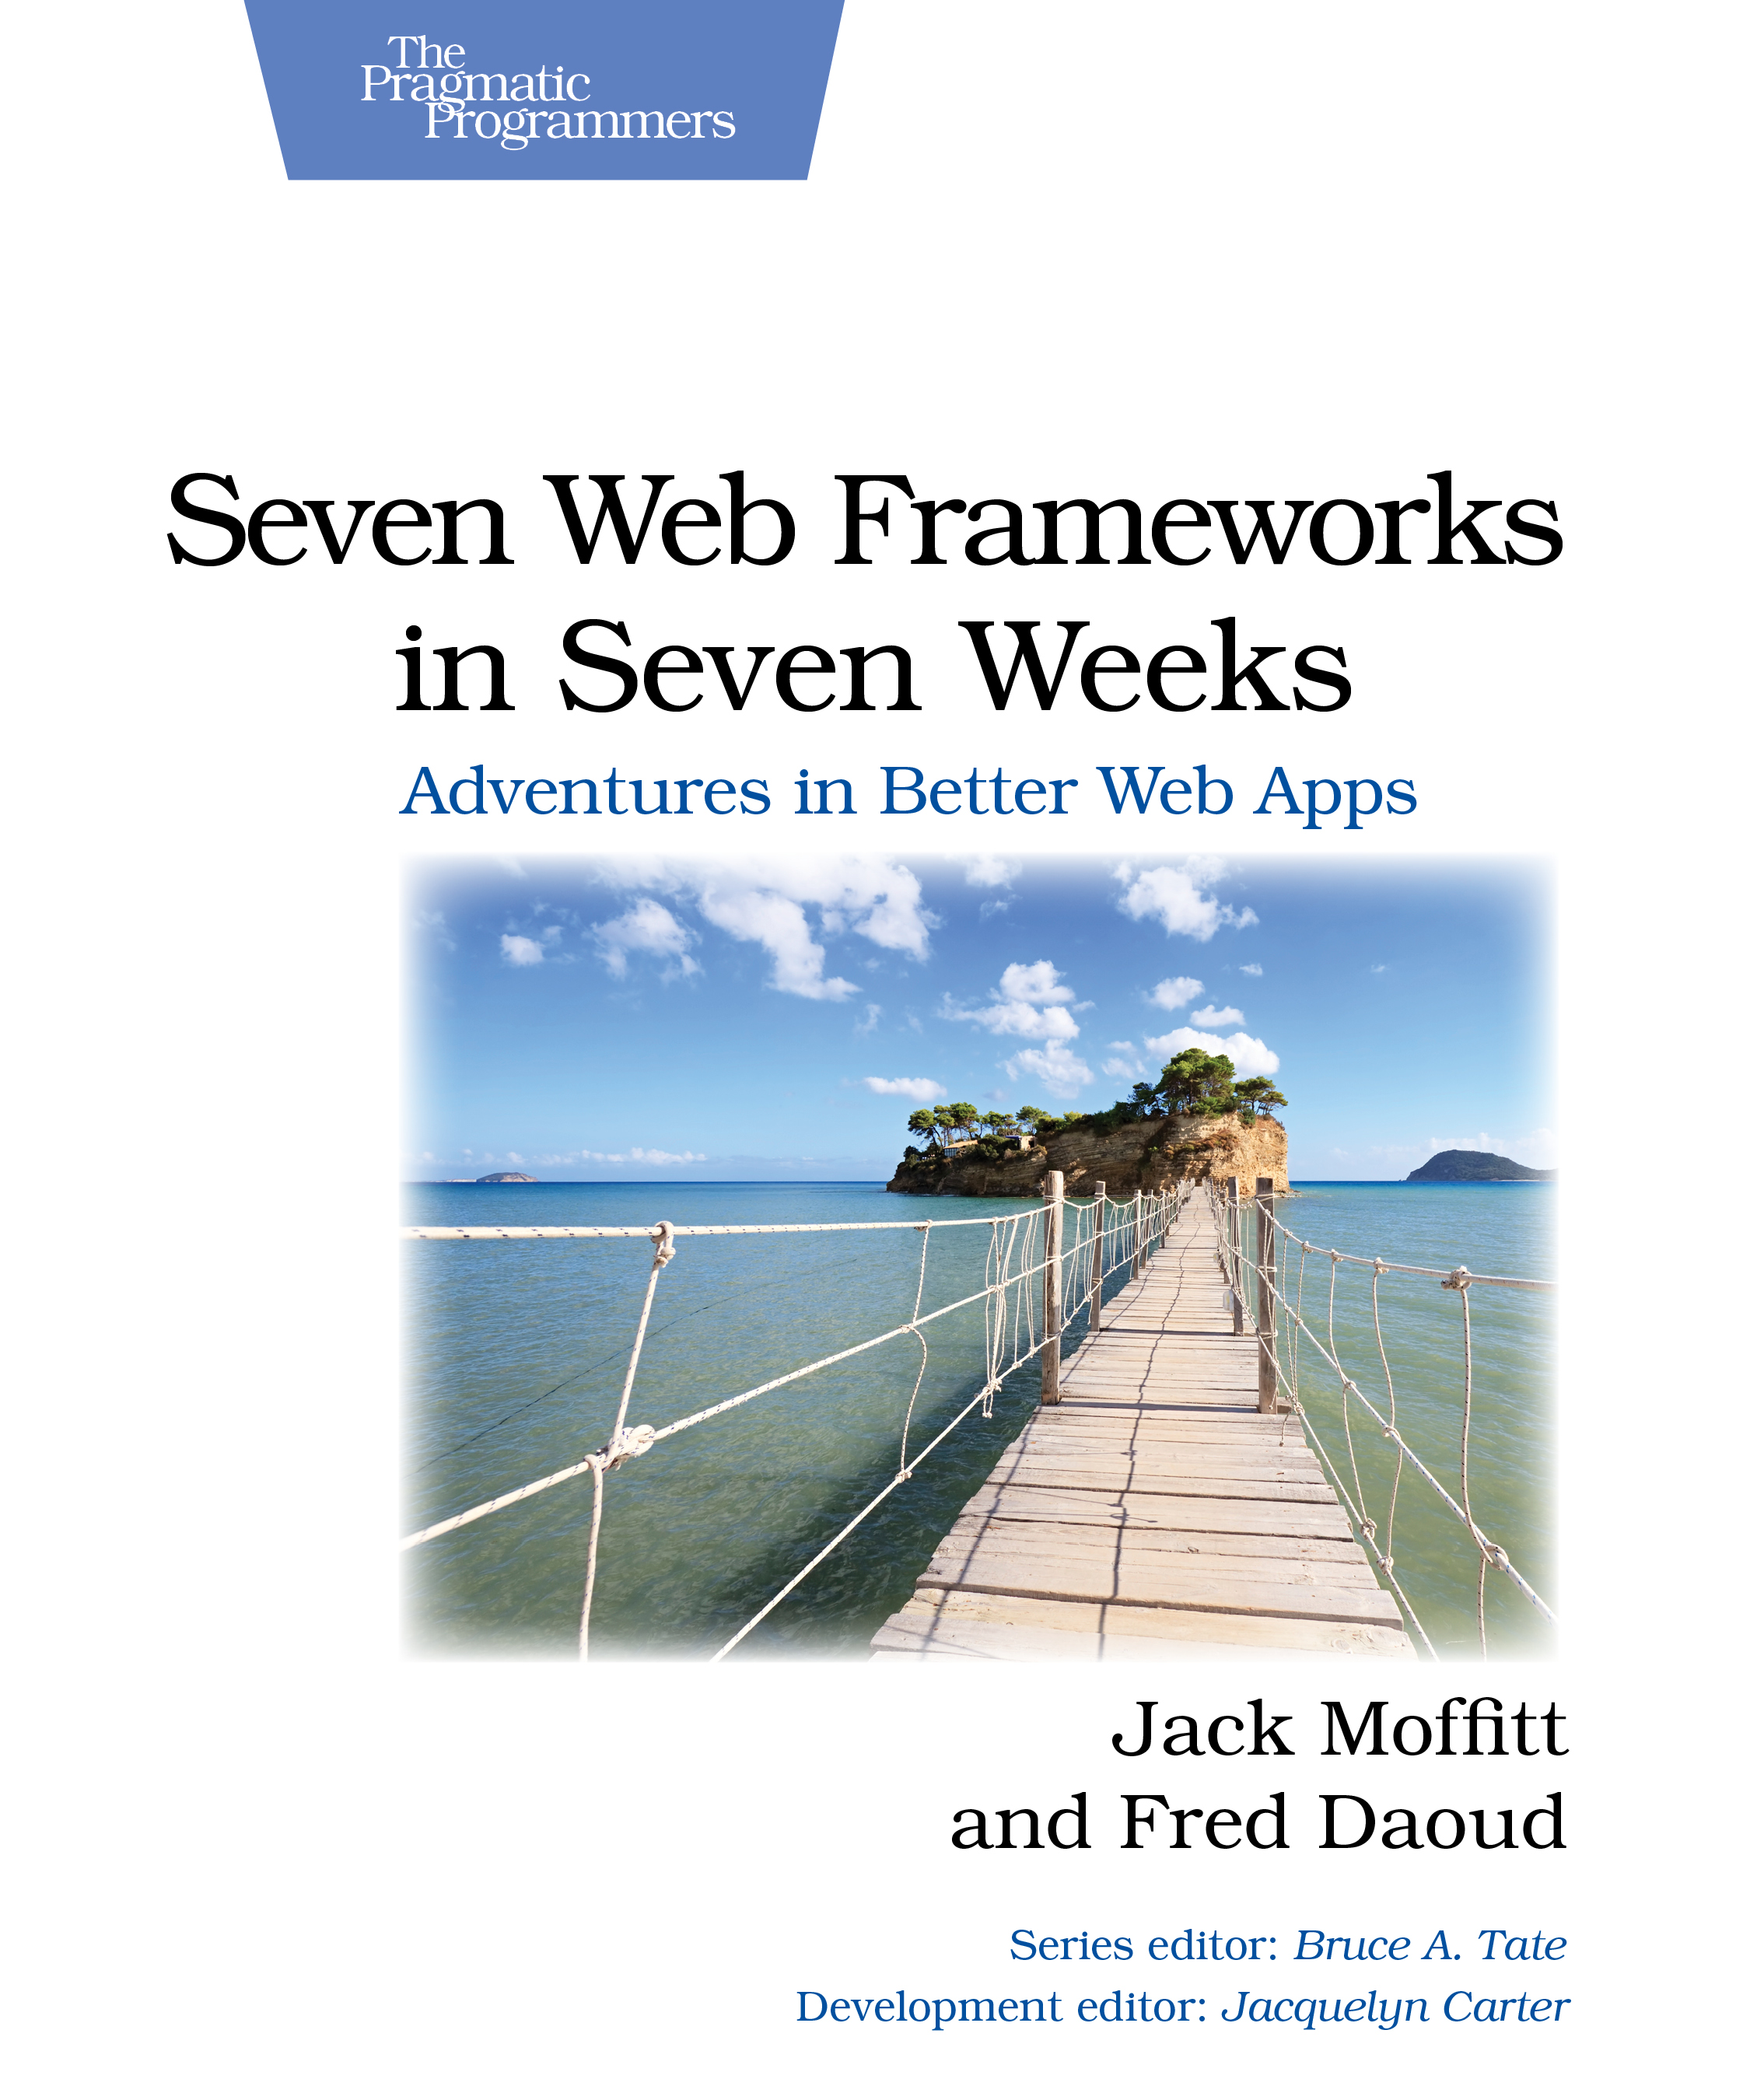
\includegraphics[width=.33\textwidth]{swfsw.jpg}}
\end{frame}

\begin{frame}
  \frametitle{Interaction between Programming Languages}
  \begin{itemize}
    \item C-based: C, C++, Go, R, Perl, Python \ldots
    \item Virtual Machine based:
    \begin{itemize}
      \item JVM: Java, Scalar, JPython, Perl 6 \ldots
      \item CLI: C++/CLI, C\#, IronPython, F\#, VB.NET, PowerShell \ldots
    \end{itemize}
    \item Interface: web service, file, database, container \ldots
  \end{itemize}
\end{frame}

\begin{frame}
  \begin{itemize}
    \item Java and R: rJava
    \item Perl and R: RSPerl
    \item Python and R: rpy2
    \item C/C++ and R: Rcpp
    \item C and Perl: perl.h
    \item Java and C/C++: JNI
  \end{itemize}
\end{frame}

\section{The World of Programming Methods}

subsection{Waterfall}
\begin{frame}
  \frametitle{Waterfall}
  \centerline{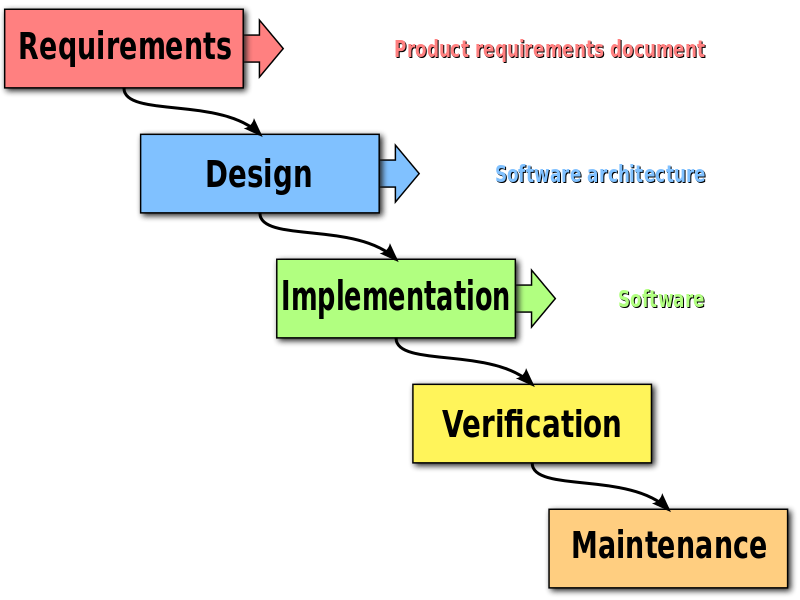
\includegraphics[height=.8\textheight]{waterflow.png}}
\end{frame}

\begin{frame}
  \frametitle{Case: Fibonacci Sequence Generator}
  \begin{itemize}
    \item Requirements: What is the input? Web based or Command line application?
    \item Design: technology stack, architecture, user experience \ldots
    \item Implementation: only coding? Construction
    \item Verification: testing, alpha, beta
    \item Maintenance:
  \end{itemize}
\end{frame}

\subsection{Agile Software Development}

\begin{frame}
  \frametitle{Agile Software Development}
  \begin{block}{Agile Software Development}
    Agile software development is a group of software development methods in which requirements and
    solutions evolve through collaboration between self-organizing, cross-functional teams. It
    promotes adaptive planning, evolutionary development, early delivery, continuous improvement
    and encourages rapid and flexible response to change.
  \end{block}
\end{frame}

\begin{frame}
  \frametitle{12 principles of agile software development}
  \tiny
  \begin{itemize}
    \item Customer satisfaction by rapid delivery of useful software
    \item Welcome changing requirements, even late in development
    \item Working software is delivered frequently (weeks rather than months)
    \item Close, daily cooperation between business people and developers
    \item Projects are built around motivated individuals, who should be trusted
    \item Face-to-face conversation is the best form of communication (co-location)
    \item Working software is the principal measure of progress
    \item Sustainable development, able to maintain a constant pace
    \item Continuous attention to technical excellence and good design
    \item Simplicity—the art of maximizing the amount of work not done—is essential
    \item Self-organizing teams
    \item Regular adaptation to changing circumstances
  \end{itemize}
\end{frame}

\begin{frame}
  \frametitle{Why do we need agile software development?}
  \begin{itemize}
    \item Stock trading system, military, bank \ldots
    \item Desktop softwares ship as floppy disk, CD or DVD \ldots
    \item Internet helps us update our software every minutes \ldots
  \end{itemize}
\end{frame}

\begin{frame}
  \begin{block}{Agile Methods}
    \begin{itemize}
      \item Extreme Programming
      \item Test Driven Programming
      \item Scrum
      \item \ldots
    \end{itemize}
  \end{block}
\end{frame}

\begin{frame}
  \begin{block}{Agile Practices}
    \begin{itemize}
      \item Pair programming
      \item test-driven
      \item story-driven modeling
      \item Iterative and incremental development
      \item Cross-functional team
      \item Refactoring
      \item \ldots
    \end{itemize}
  \end{block}
\end{frame}

\section{The World of Programming Tools}

\subsection{Source Version Control}

\begin{frame}[t]{git}
    git
\end{frame}
%--- Next Frame ---%

\begin{frame}[t]{Subversion}
    svn
\end{frame}
%--- Next Frame ---%

\begin{frame}[t]{Hosted SVC}
    github
    bitbucket
    coding.net
\end{frame}
%--- Next Frame ---%

\subsection{Teamwork}
\begin{frame}[t]{Communication}
    Slask
\end{frame}
%--- Next Frame ---%

\begin{frame}[t]{Project Management}
    Trell
    Tower.im
    Worktitle
\end{frame}
%--- Next Frame ---%

\subsection{Documentation}

\subsection{Deployment}

\subsection{Other}

\begin{frame}
  \centerline{\Huge{Thanks!}}
\end{frame}
%--- Next Frame ---%

\end{document}
